\documentclass[final]{beamer}

\usepackage[T1]{fontenc}
\usepackage[utf8]{inputenc}
\usepackage[spanish,es-noquoting,es-nolists,es-noshorthands]{babel}
\usepackage{lmodern}
\usepackage[orientation=portrait,size=a0,scale=1.9]{beamerposter}
\usepackage{amsmath,amssymb}
\usepackage{booktabs}
\graphicspath{{figuras/}{../entrega-final/figuras/}}

\definecolor{tinta}{HTML}{1F2933}
\definecolor{acento}{HTML}{2A78D6}
\definecolor{suave}{HTML}{6B7280}
\definecolor{fondo}{HTML}{F3F6FA}
\setbeamercolor{normal text}{fg=tinta,bg=white}
\setbeamercolor{structure}{fg=acento}
\setbeamercolor{block title}{fg=white,bg=acento}
\setbeamercolor{block body}{fg=tinta,bg=fondo}
\setbeamerfont{block title}{size=\Large,series=\bfseries}
\setbeamertemplate{navigation symbols}{}
\setbeamertemplate{itemize items}{\color{acento}\textbullet}
\setbeamertemplate{blocks}[rounded][shadow=false]
\newcommand{\clave}[1]{{\color{acento}\bfseries #1}}
\setlength{\parskip}{0.4ex}
\addtobeamertemplate{block end}{}{\vspace{1.6ex}}

\begin{document}
\begin{frame}[t]

% ------------------------------------------------------------------ cabecera
\begin{center}
{\fontsize{120}{140}\selectfont\bfseries Estructura frente a tamaño}\\[1ex]
{\fontsize{64}{76}\selectfont Selección de conjuntos críticos en el grafo de exposición de DeFi}\\[1.2ex]
{\Large David Sánchez Lombana \quad·\quad Juan Sebastián Cuesta Montenegro}\\[0.4ex]
{\large\color{suave} Teoría de Grafos 2026-II · Prof.\ Daniel Bojacá · Universidad del Rosario}
\end{center}
\vspace{1ex}
{\color{acento}\rule{\linewidth}{4pt}}
\vspace{1ex}

\begin{columns}[t,totalwidth=\linewidth]

% ------------------------------------------------------------------ columna 1
\begin{column}{0.31\linewidth}

\begin{block}{Pregunta}
Los protocolos DeFi reutilizan los mismos activos como colateral: la caída de
uno se propaga. El estado del arte elige qué protocolos estresar \clave{por
tamaño}.

\vspace{0.5ex}
\textbf{Con un presupuesto de $k$ protocolos, ¿qué conjunto fragmenta más la
red, y lo encuentran mejor los criterios estructurales o los de tamaño?}
\end{block}

\begin{block}{Modelo}
\begin{itemize}
\item Panel público de DeXposure: 314 semanas, $u\to v$ si $u$ depende de $v$,
      peso en USD.
\item Proyección no dirigida, componente gigante $C_t$ (98--99{,}8\,\% de los
      vértices). Problema NP-duro: heurísticas.
\item Dos medidas de daño:
\end{itemize}
\[
R_{\mathrm{est}}=\frac{\max_Q|Q|}{|C_t|},\qquad L=1-R
\]
\[
R_{\mathrm{pond}}=\frac{\max_Q W_t(Q)}{W_0}
\]
\[
L_{\mathrm{pond}}=L_{\mathrm{directa}}+L_{\mathrm{frag}}
\]
\end{block}

\begin{block}{Reglas y protocolo}
\textbf{Tamaño:} fuerza de exposición, PageRank.\\
\textbf{Estructura:} intermediación, articulación adaptativa, CDS de
Guha--Khuller, inmunización espectral exacta.\\
\textbf{Controles:} voraz sin restricción, aleatorio, TVL/SIS (exploratorio).

\vspace{0.5ex}
13 semanas fijadas de antemano (un trimestre de 2022--2024 y las previas a
Terra/Luna, FTX y USDC), $k\in\{1,2,5,10,20\}$.
\end{block}

\begin{block}{Resultados teóricos}
\begin{itemize}
\item \clave{Lema de las hojas}: hay un óptimo sin hojas.
\item Articulación \clave{óptima para $k=1$} en $L_{\mathrm{est}}$.
\item $L_{\mathrm{directa}}$ \clave{submodular}: voraz $\geq(1-1/e)$ del óptimo.
\item $\rho(A)=\max_{\text{SCC}}\rho$ (Frobenius).
\end{itemize}
\end{block}

\end{column}

% ------------------------------------------------------------------ columna 2
\begin{column}{0.36\linewidth}

\begin{block}{Cada familia gana en lo que optimiza}
\centering
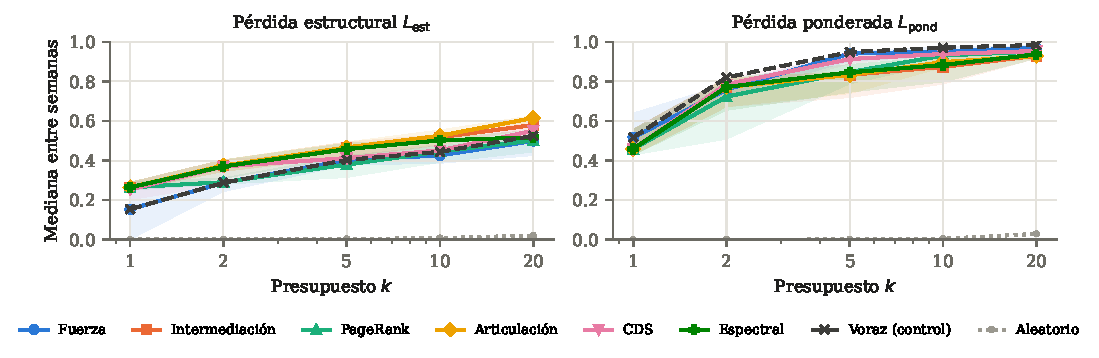
\includegraphics[width=\linewidth]{fig_curvas.pdf}

\vspace{0.5ex}
\raggedright
\resizebox{\linewidth}{!}{%
\begin{tabular}{lcccccc}
\toprule
$k=10$ & $L_{\mathrm{est}}$ & gana & $L_{\mathrm{pond}}$ & gana & $F_{\mathrm{rel}}$ & gana \\
\midrule
Fuerza         & 0{,}43 & 0/0 & 0{,}95 & 0/7 & 0{,}011 & 0/8 \\
Intermediación & 0{,}52 & 1/9 & 0{,}87 & 0/0 & 0{,}009 & 1/7 \\
PageRank       & 0{,}45 & 0/0 & 0{,}93 & 0/0 & 0{,}010 & 1/7 \\
Articulación   & \textbf{0{,}53} & \textbf{13/13} & 0{,}90 & 0/0 & 0{,}010 & 1/8 \\
CDS            & 0{,}45 & 0/0 & 0{,}94 & 0/4 & 0{,}016 & 3/10 \\
Espectral      & 0{,}50 & 0/0 & 0{,}88 & 0/0 & 0{,}016 & 0/8 \\
Voraz          & 0{,}44 & 0/0 & \textbf{0{,}97} & \textbf{13/13} & 0{,}016 & 7/10 \\
\bottomrule
\end{tabular}}

\vspace{0.3ex}
{\small Medianas; gana = estrictas / a menos de 0{,}01. Victorias \clave{en parte circulares}: cada regla gana en lo que optimiza. Con $F_{\mathrm{rel}}$, que nadie optimiza, ninguna domina.}
\end{block}

\begin{block}{De qué está hecho el daño}
\centering
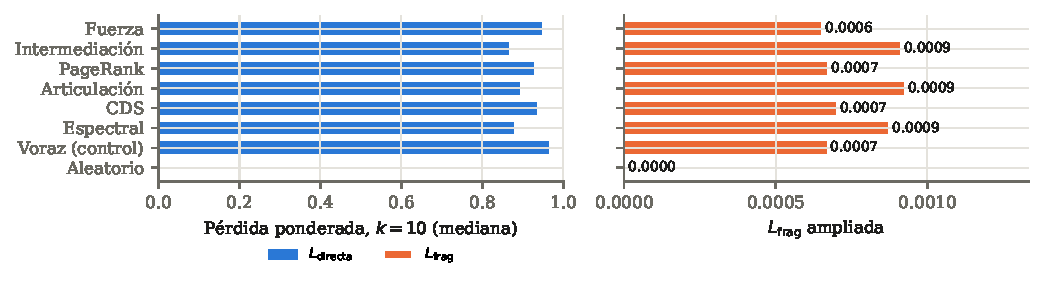
\includegraphics[width=\linewidth]{fig_descomposicion.pdf}

\raggedright
$L_{\mathrm{frag}}\le0{,}009$ siempre: la exposición se pierde quitando, no
partiendo. El 84\,\% del $L_{\mathrm{est}}$ de la articulación son \clave{hojas
aisladas}; en fragmentos $\geq2$ su ventaja sobre la fuerza es de 3 puntos.
\end{block}

\begin{block}{Dos familias de conjuntos}
\begin{columns}[c]
\column{0.55\linewidth}
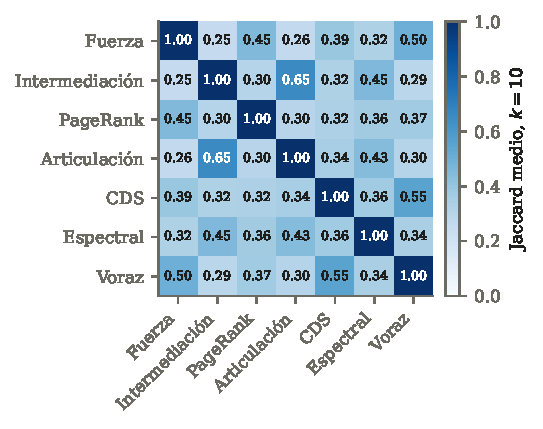
\includegraphics[width=\linewidth]{fig_jaccard.pdf}
\column{0.45\linewidth}
Jaccard fuerza--articulación 0{,}26; intermediación--articulación 0{,}65.
El conjunto estructuralmente crítico \clave{no} es el de los más grandes.
\end{columns}
\end{block}

\begin{block}{Herramienta \texttt{critset}}
\begin{itemize}
\item CLI reproducible (uv); articulación en $O(n+m)$ por paso (Tarjan).
\item 48 pruebas contra NetworkX y fuerza bruta.
\end{itemize}
\end{block}

\end{column}

% ------------------------------------------------------------------ columna 3
\begin{column}{0.31\linewidth}

\begin{block}{Sensibilidad ($k=10$, $L_{\mathrm{est}}$ / $L_{\mathrm{pond}}$)}
\centering
\resizebox{\linewidth}{!}{%
\begin{tabular}{lccc}
\toprule
 & Sin \emph{Unk.} & Sin no prot. & 2-núcleo \\
\midrule
Fuerza       & 0{,}21/0{,}92 & 0{,}11/0{,}69 & 0{,}22/0{,}96 \\
Articulación & \textbf{0{,}38}/0{,}83 & \textbf{0{,}30}/0{,}51 & \textbf{0{,}30}/0{,}90 \\
CDS          & 0{,}25/0{,}90 & 0{,}22/0{,}75 & 0{,}21/0{,}90 \\
Voraz        & 0{,}24/\textbf{0{,}94} & 0{,}19/\textbf{0{,}77} & 0{,}22/\textbf{0{,}97} \\
\bottomrule
\end{tabular}}

\raggedright
Sin \emph{Unknown}, sin cadenas ni exchanges, y sin hojas: \clave{el patrón se mantiene}.
\end{block}

\begin{block}{Costo computacional}
\centering
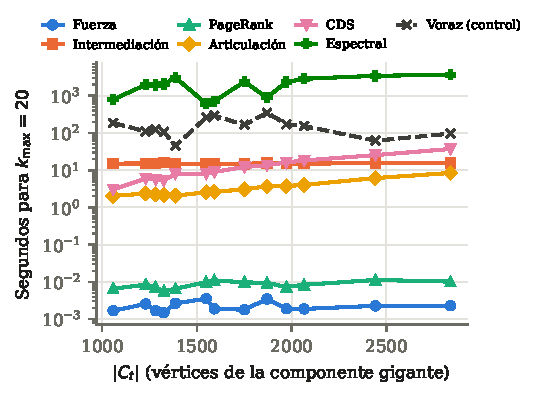
\includegraphics[width=0.9\linewidth]{fig_tiempos.pdf}

\raggedright
De milisegundos (fuerza, PageRank) a una hora (espectral exacta, $k=20$).
Todas viables para monitoreo semanal.
\end{block}

\begin{block}{Episodios y límites}
\begin{itemize}
\item Indicador de afectación (caída de al menos 50\,\% en 4 semanas): tasa base
      47--67\,\%. Ninguna regla la supera en los tres episodios:
      \clave{resultado nulo}.
\item El TVL publicado no cubre $C_t$: TVL (0{,}52--0{,}67) y SIS (0{,}62--0{,}91
      de $L_{\mathrm{pond}}$) quedan como exploratorios.
\end{itemize}
\end{block}

\begin{block}{Conclusiones}
\begin{itemize}
\item Cada familia gana en la medida que optimiza; el daño estructural es
      sobre todo \clave{aislar hojas}.
\item Ninguna regla parte la exposición: en promedio queda más del 94\,\% en una componente.
\item El CDS no supera al voraz sin restricción.
\item Pendiente: modelo nulo, reglas adaptativas, $k=2$ exacto, DebtRank.
\end{itemize}
\end{block}

\end{column}
\end{columns}

\end{frame}
\end{document}
